
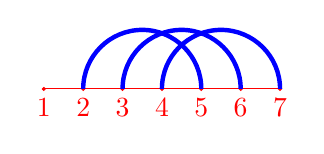
\begin{tikzpicture}[scale=0.5]
\centering
\label{staircasedecompisition}

\foreach \i in {1,...,6} {
        \draw[red] (\i,1) -- (\i + 1,1)node[pos=0.0,below] {\i};
        \filldraw[red] (\i,1) circle (1pt);
 }

\draw[red] (7,1) -- (6,1)node[pos=0.0,below] {7};
\filldraw[red] (7,1) circle (1pt);

\draw[blue, ultra thick] (2,1) arc(180:0:1.5);
\draw[blue, ultra thick] (3,1) arc(180:0:1.5);
\draw[blue, ultra thick] (4,1) arc(180:0:1.5);
\end{tikzpicture}